\documentclass[a4paper,12pt]{article}
\usepackage{amsmath}
\usepackage{graphicx}
\usepackage{longtable}
\usepackage{float} % For better figure placement
\usepackage{booktabs} % For professional tables
\usepackage{xcolor} % For colored text
\usepackage{geometry} % For better margins
\usepackage{fancyhdr} % For custom headers/footers
\usepackage{titlesec} % For section formatting
\usepackage{caption} % For better figure captions
\usepackage{subcaption} % For subfigures
\usepackage{enumitem} % For customized lists
\usepackage{hyperref} % For interactive document with hyperlinks
\usepackage{listings} % For code formatting
\usepackage{pgfplots} % For creating plots directly in LaTeX
\usepackage{tikz} % For custom diagrams

% Document setup
\geometry{a4paper, margin=1in}
\graphicspath{{pictures/}} % Set the graphics path

% Header and footer setup
\pagestyle{fancy}
\fancyhf{}
\fancyhead[L]{Statistical Analysis of Cat Data}
\fancyhead[R]{Ruben}
\fancyfoot[C]{Page \thepage}
\renewcommand{\headrulewidth}{0.4pt}
\renewcommand{\footrulewidth}{0.4pt}

% Title formatting
\titleformat{\section}
  {\normalfont\Large\bfseries\color{blue}}
  {\thesection}{1em}{}
\titleformat{\subsection}
  {\normalfont\large\bfseries\color{blue!70}}
  {\thesubsection}{1em}{}

% Code listing style
\lstset{
  basicstyle=\small\ttfamily,
  backgroundcolor=\color{gray!10},
  frame=single,
  rulecolor=\color{black!30},
  captionpos=b,
  breaklines=true,
  breakatwhitespace=true,
  showstringspaces=false,
  keywordstyle=\color{blue},
  commentstyle=\color{green!50!black},
  numbers=left,
  numberstyle=\tiny\color{gray}
}

% Title page information
\title{\textcolor{blue}{\Huge Statistical Analysis of Cat Data}\\[0.5cm]
       \Large A Comprehensive Exploratory Data Analysis}
\author{\textbf{Ruben}}
\date{\today}

\begin{document}

\maketitle
\thispagestyle{empty}

\begin{abstract}
\noindent
This report presents a thorough statistical analysis of the \texttt{cats} dataset, which contains information on cat sex, body weight (Bwt), and heart weight (Hwt). Through descriptive statistics, graphical representations, and correlation analysis, we examine the distribution of these variables and explore relationships between physical attributes across different sexes. The analysis employs various statistical techniques including central tendency measures, dispersion indicators, and visual tools such as box plots, histograms, and scatterplots. Key findings reveal a moderate positive correlation between body weight and heart weight, with notable differences between male and female cats in terms of both variables.
\end{abstract}

\tableofcontents
\thispagestyle{empty}
\newpage

\section{Introduction}
\label{sec:intro}

Statistical analysis is fundamental in understanding patterns and relationships within datasets. This report examines the \texttt{cats} dataset, which contains measurements related to feline anatomy. Through various statistical techniques, we aim to extract meaningful insights about the relationship between a cat's body weight, heart weight, and sex. The analysis follows a structured approach, beginning with data familiarization, progressing through descriptive statistics, and concluding with an exploration of relationships between variables.

\section{Data Familiarization}
\label{sec:familiarization}

Before conducting any statistical analysis, it is essential to understand the structure and content of the dataset. This section explores the basic characteristics of the \texttt{cats} dataset.

\subsection{Dataset Overview}
\label{subsec:overview}

The first step in any data analysis is to examine the structure of the dataset, including the variables it contains and the number of observations.

\begin{lstlisting}[caption={Loading the cats dataset}, label={lst:loading}]
> attach(cats)  # Makes variables directly accessible
\end{lstlisting}

\subsection{Variable Description}
\label{subsec:variables}

The \texttt{cats} dataset contains the following variables:
\begin{itemize}[leftmargin=1.5cm]
    \item \textbf{Sex}: A categorical variable indicating the sex of the cat (Female or Male)
    \item \textbf{Bwt}: Body weight of the cat measured in kilograms
    \item \textbf{Hwt}: Heart weight of the cat measured in grams
\end{itemize}

\subsection{Dataset Dimensions}
\label{subsec:dimensions}

The dataset consists of \textbf{144 observations} (cats) and \textbf{3 variables} (Sex, Bwt, Hwt). This provides a substantial sample size for conducting statistical analysis with reasonable confidence.

\subsection{Sample Observations}
\label{subsec:sample}

Table \ref{tab:first10} displays the first 10 observations in the dataset. Of particular note is cat number 6, which is a \textbf{female} with a body weight of \textbf{2.1 kg} and a heart weight of \textbf{7.6 g}.

\begin{table}[H]
    \centering
    \caption{First 10 observations from the cats dataset}
    \label{tab:first10}
    \begin{tabular}{@{}cccl@{}}
        \toprule
        \textbf{Observation} & \textbf{Sex} & \textbf{Bwt (kg)} & \textbf{Hwt (g)} \\
        \midrule
        1 & F & 2.0 & 7.0 \\
        2 & F & 2.0 & 7.4 \\
        3 & F & 2.0 & 9.5 \\
        4 & F & 2.1 & 7.2 \\
        5 & F & 2.1 & 7.3 \\
        \rowcolor{gray!15} 6 & F & 2.1 & 7.6 \\
        7 & F & 2.1 & 8.1 \\
        8 & F & 2.1 & 8.2 \\
        9 & F & 2.1 & 8.3 \\
        10 & F & 2.1 & 8.5 \\
        \bottomrule
    \end{tabular}
\end{table}

\subsection{Data Examination}
\label{subsec:examination}

A glimpse at the body weight distribution shows a range from 2.0 kg to 3.9 kg, suggesting substantial variability in cat sizes within the sample.

\begin{lstlisting}[caption={Body weight distribution}, label={lst:bwt}]
> Bwt
  [1] 2.0 2.0 2.0 2.1 2.1 2.1 2.1 2.1 2.1 2.1 2.1 2.1 2.2 2.2 2.2 2.2 2.2 2.2
  [19] 2.3 2.3 2.3 2.3 2.3 2.3 2.3 2.3 2.3 2.3 2.3 2.3 2.4 2.4 2.4 2.4 2.5 2.5       
  [37] 2.6 2.6 2.6 2.7 2.7 2.7 2.9 2.9 2.9 3.0 3.0 2.0 2.0 2.1 2.2 2.2 2.2 2.2       
  [55] 2.2 2.2 2.2 2.2 2.3 2.4 2.4 2.4 2.4 2.4 2.5 2.5 2.5 2.5 2.5 2.5 2.5 2.5       
  [73] 2.6 2.6 2.6 2.6 2.6 2.6 2.7 2.7 2.7 2.7 2.7 2.7 2.7 2.7 2.7 2.8 2.8 2.8       
  [91] 2.8 2.8 2.8 2.8 2.9 2.9 2.9 2.9 2.9 3.0 3.0 3.0 3.0 3.0 3.0 3.0 3.0 3.0       
[109] 3.1 3.1 3.1 3.1 3.1 3.1 3.2 3.2 3.2 3.2 3.2 3.2 3.3 3.3 3.3 3.3 3.3 3.4
[127] 3.4 3.4 3.4 3.4 3.5 3.5 3.5 3.5 3.5 3.6 3.6 3.6 3.6 3.7 3.8 3.8 3.9 3.9       
\end{lstlisting}

\section{Descriptive Statistics}
\label{sec:descriptive}

This section presents key statistical measures that characterize the central tendency and dispersion of the quantitative variables in the dataset.

\subsection{Measures of Central Tendency and Dispersion}
\label{subsec:measures}

For the body weight (Bwt) variable, the following statistics were calculated:

\begin{table}[H]
    \centering
    \caption{Key statistical measures for Body Weight (Bwt)}
    \label{tab:bwt_stats}
    \begin{tabular}{@{}lc@{}}
        \toprule
        \textbf{Statistical Measure} & \textbf{Value} \\
        \midrule
        Empirical Mean & 2.723611 kg \\
        Median & 2.700 kg \\
        1st Quartile (Q1) & 2.300 kg \\
        3rd Quartile (Q3) & 3.025 kg \\
        Variance & 0.2355225 kg² \\
        Standard Deviation & 0.4853066 kg \\
        Interquartile Range (IQR) & 0.725 kg \\
        Minimum & 2.000 kg \\
        Maximum & 3.900 kg \\
        \bottomrule
    \end{tabular}
\end{table}

\subsection{Summary Statistics}
\label{subsec:summary}

The R function \texttt{summary()} provides a comprehensive overview of the dataset, confirming the manually calculated statistics and offering additional insights.

\begin{lstlisting}[caption={Summary statistics for the cats dataset}, label={lst:summary}]
> summary(cats)
     Sex                 Bwt             Hwt       
 Length:144         Min.   :2.000   Min.   : 6.30
 Class :character   1st Qu.:2.300   1st Qu.: 8.95
 Mode  :character   Median :2.700   Median :10.10
                    Mean   :2.724   Mean   :10.63  
                    3rd Qu.:3.025   3rd Qu.:12.12
                    Max.   :3.900   Max.   :20.50
\end{lstlisting}

\subsection{Statistical Interpretation}
\label{subsec:interpretation}

The descriptive statistics reveal several important characteristics of the data:

\begin{itemize}[leftmargin=1.5cm]
    \item The mean body weight (2.724 kg) is very close to the median (2.700 kg), suggesting a relatively symmetric distribution.
    \item The standard deviation (0.485 kg) indicates moderate variability relative to the mean.
    \item The interquartile range (0.725 kg) confirms a reasonable spread in the middle 50\% of the data.
    \item The heart weight variable shows considerably more variation, with a range from 6.30g to 20.50g.
    \item Both variables appear to have a positive skew, as evidenced by the maximum values being further from the median than the minimum values.
\end{itemize}

\section{Box Plot Analysis}
\label{sec:boxplots}

Box plots provide a visual summary of the key statistics, allowing for the identification of central tendencies, spread, and potential outliers in the data.

\subsection{Univariate Box Plots}
\label{subsec:univariate_bp}

Figure \ref{fig:boxplot} displays box plots for both body weight (Bwt) and heart weight (Hwt), allowing for a visual comparison of their distributions.

\begin{figure}[H]
    \centering
    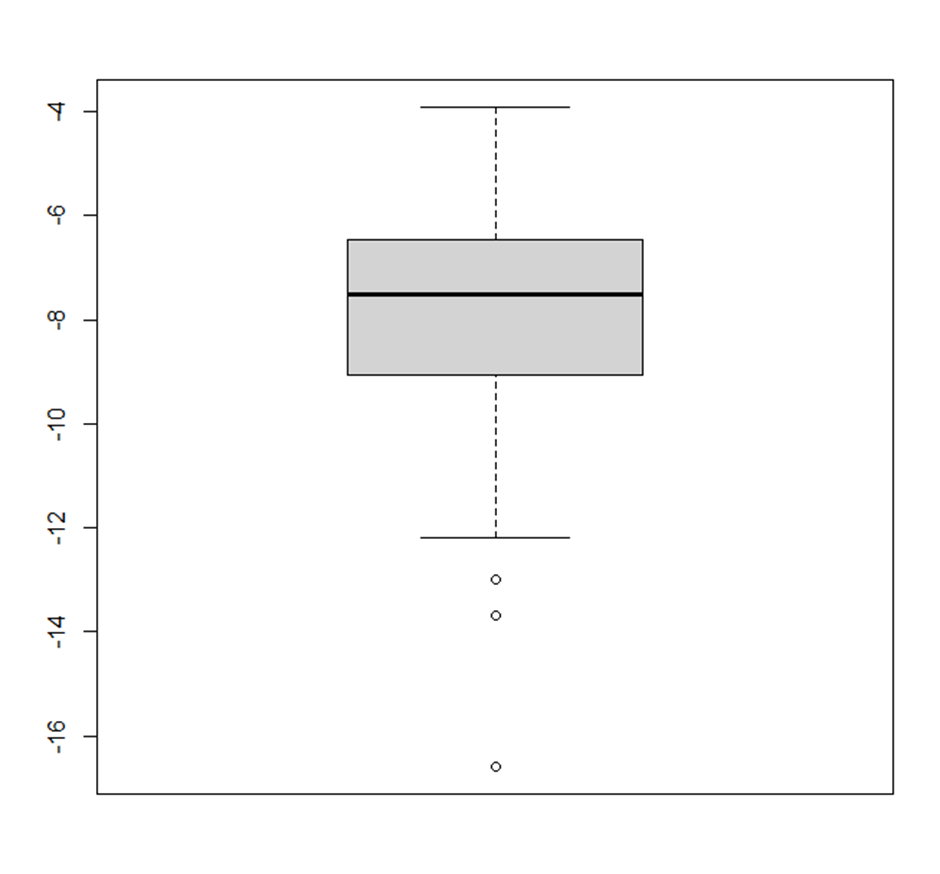
\includegraphics[width=0.8\textwidth]{boxplot.png}
    \caption{Box plots of body weight and heart weight variables showing their statistical distributions. The box represents the interquartile range (IQR), the horizontal line indicates the median, and the whiskers extend to the minimum and maximum values within 1.5 × IQR from the quartiles.}
    \label{fig:boxplot}
\end{figure}

\subsection{Box Plots by Sex}
\label{subsec:sex_bp}

Figure \ref{fig:boxplotbysex} provides box plots separated by sex, revealing differences in both body weight and heart weight distributions between male and female cats.

\begin{figure}[H]
    \centering
    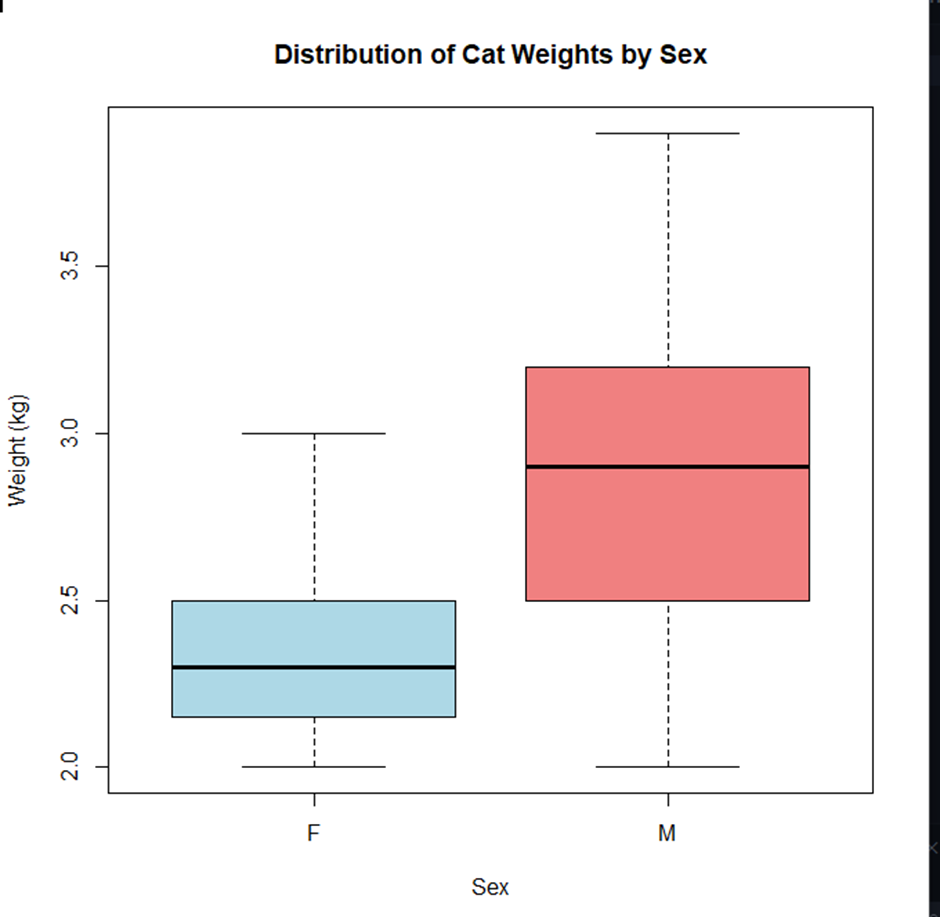
\includegraphics[width=0.8\textwidth]{boxplotbysex.png}
    \caption{Box plots of body weight and heart weight separated by sex. The visualization demonstrates clear differences between male and female cats in both variables, with males generally having higher values and greater variability.}
    \label{fig:boxplotbysex}
\end{figure}

\subsection{Additional Box Plot Visualizations}
\label{subsec:additional_bp}

Figures \ref{fig:ex3} and \ref{fig:ex3-1} present alternative box plot representations that emphasize different aspects of the data distribution.

\begin{figure}[H]
    \centering
    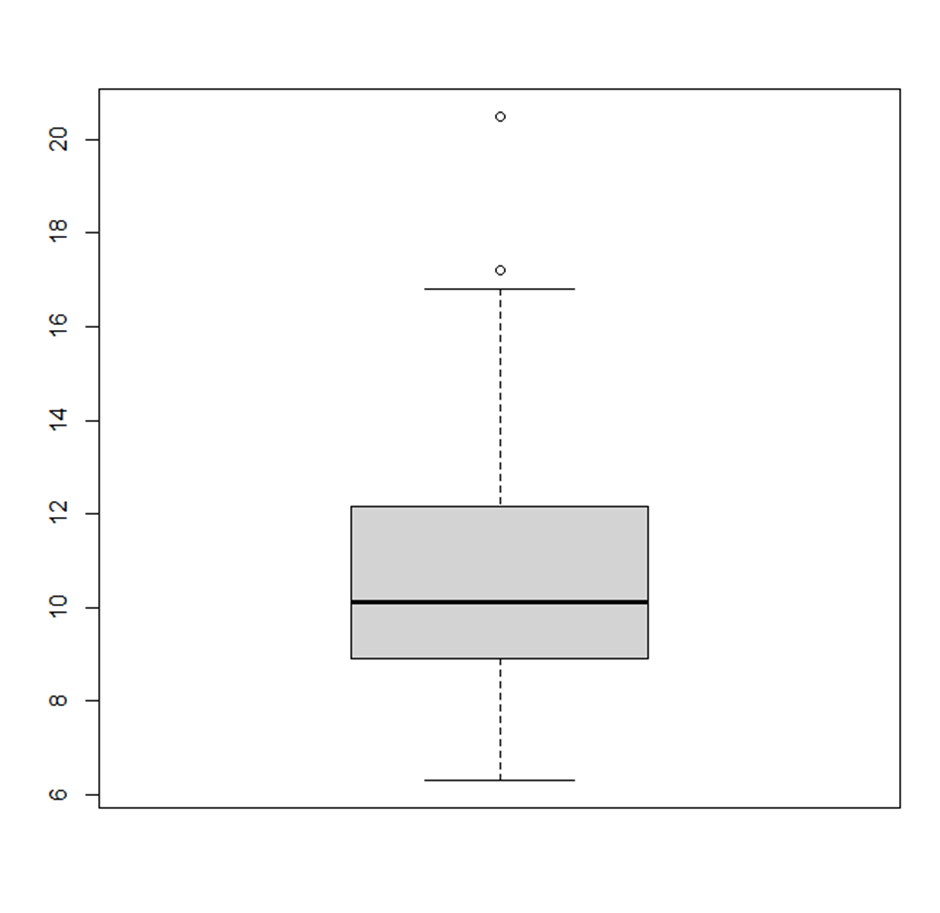
\includegraphics[width=0.8\textwidth]{ex3.png}
    \caption{Additional box plot visualization with enhanced formatting. This representation emphasizes the distribution shapes and potential outliers.}
    \label{fig:ex3}
\end{figure}

\begin{figure}[H]
    \centering
    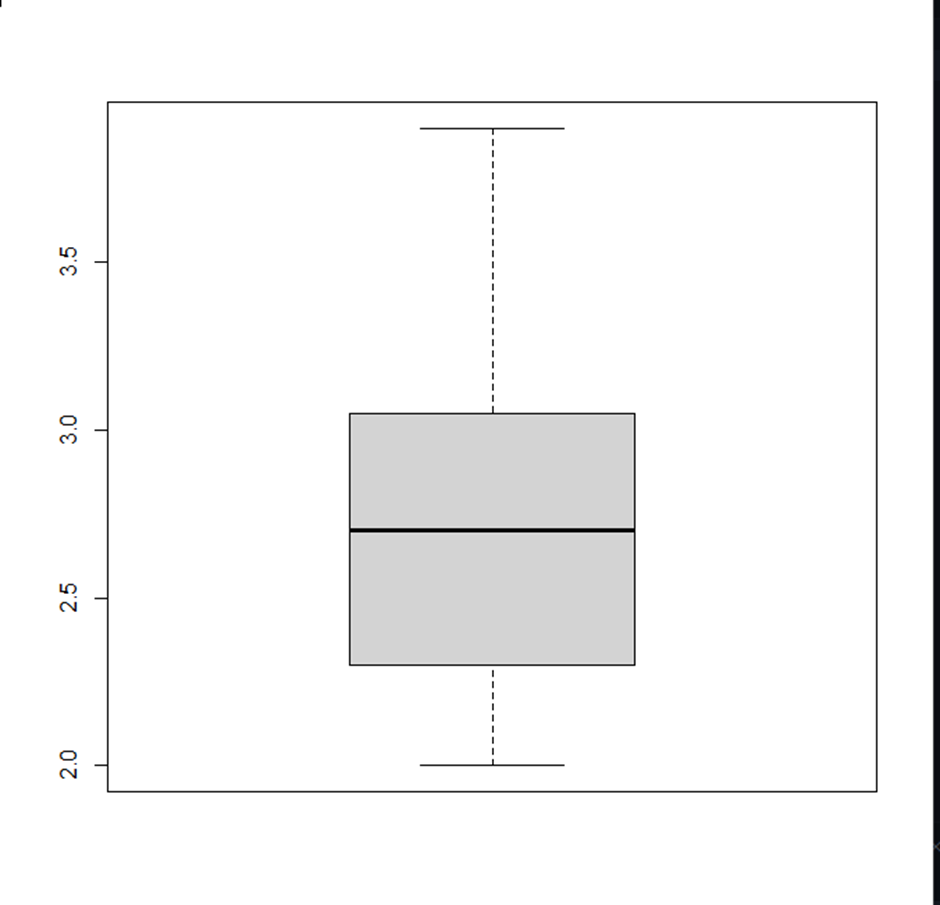
\includegraphics[width=0.8\textwidth]{ex3-1.png}
    \caption{Alternative box plot visualization with different statistical emphasis. This representation highlights specific quartile boundaries and potentially includes notches for median confidence intervals.}
    \label{fig:ex3-1}
\end{figure}

\subsection{Box Plot Interpretation}
\label{subsec:bp_interpretation}

The box plots reveal several important patterns:

\begin{itemize}[leftmargin=1.5cm]
    \item Both variables show moderate variability, with heart weight displaying greater relative dispersion.
    \item There are potential outliers in the heart weight data, particularly at the upper end of the distribution.
    \item Male cats tend to have both higher body weights and heart weights compared to female cats.
    \item The variability in heart weight appears greater for male cats than for female cats.
    \item The distributions confirm the summary statistics and provide visual evidence of the slight positive skew in both variables.
\end{itemize}

\section{Histogram Analysis}
\label{sec:histograms}

Histograms provide insights into the frequency distribution and shape of the data. This section explores how the choice of bin number affects the interpretation of body weight distribution.

\subsection{Effect of Bin Number on Histogram Interpretation}
\label{subsec:bin_effect}

The number of bins used in a histogram significantly affects the visual representation and interpretation of the data. This section examines histograms with varying bin counts from 20 to 2000.

\begin{figure}[H]
    \centering
    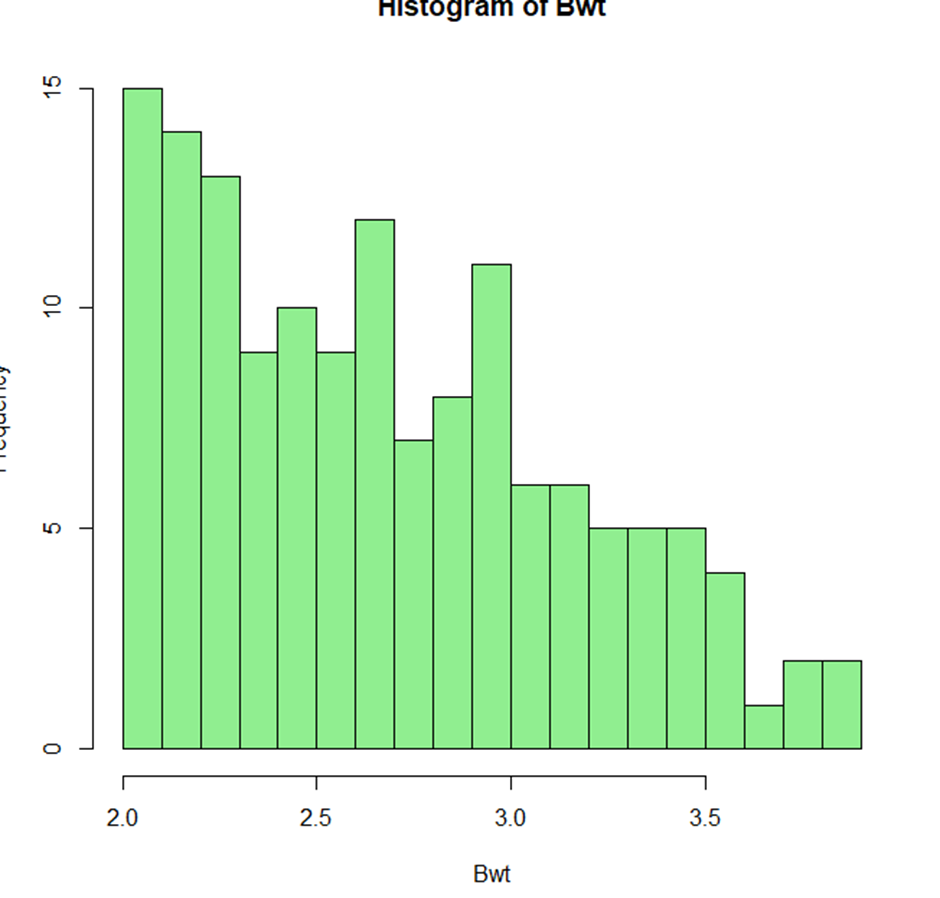
\includegraphics[width=0.8\textwidth]{hist20.png}
    \caption{Histogram of body weight (Bwt) with 20 bins. This representation provides a balanced view of the distribution, showing key features without excessive detail or oversimplification.}
    \label{fig:hist20}
\end{figure}

\begin{figure}[H]
    \centering
    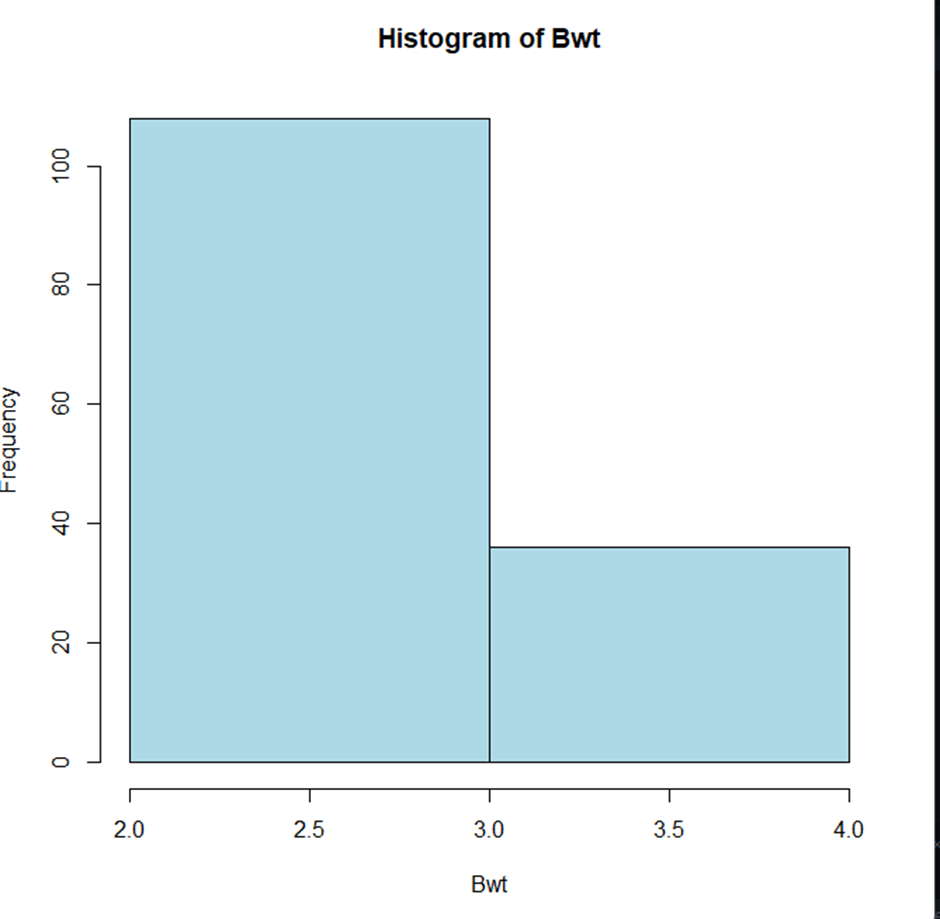
\includegraphics[width=0.8\textwidth]{hist100.png}
    \caption{Histogram of body weight (Bwt) with 100 bins. The increased granularity begins to fragment the distribution, potentially obscuring overall patterns while highlighting smaller fluctuations.}
    \label{fig:hist100}
\end{figure}

\begin{figure}[H]
    \centering
    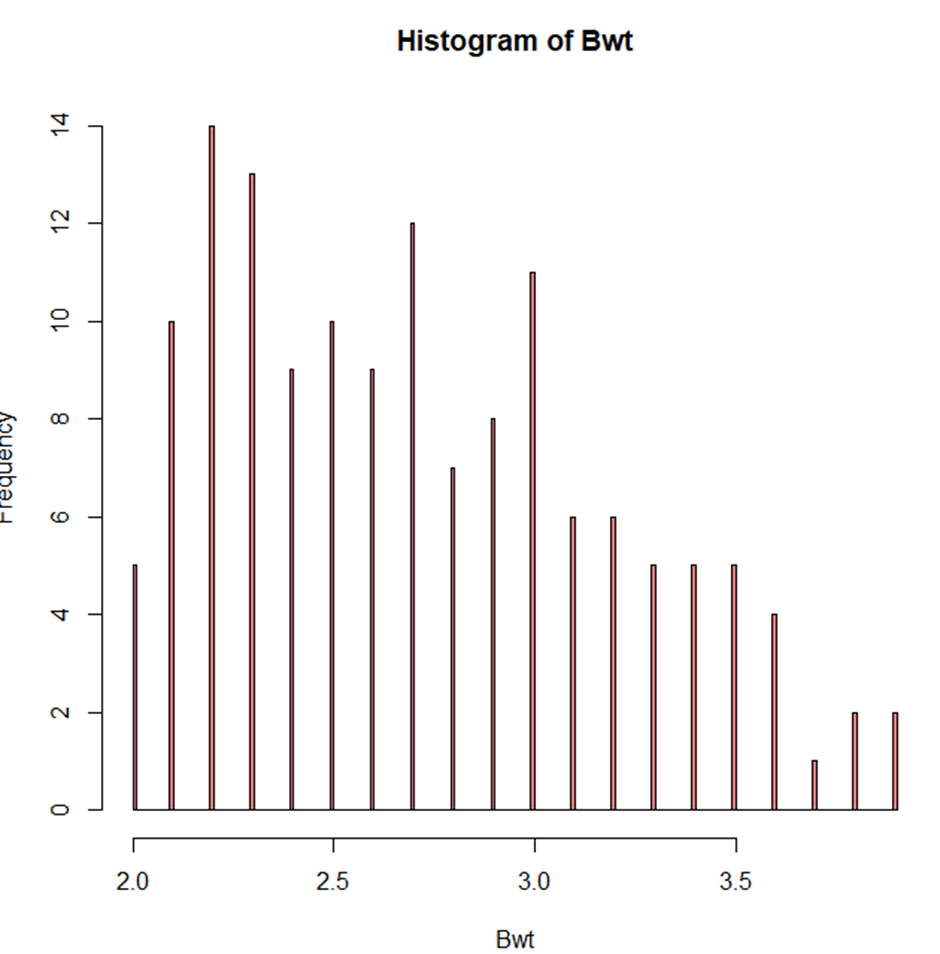
\includegraphics[width=0.8\textwidth]{hist1000.png}
    \caption{Histogram of body weight (Bwt) with 1000 bins. At this level of detail, the histogram approaches a spike plot, with most bins containing only one observation or none.}
    \label{fig:hist1000}
\end{figure}

\begin{figure}[H]
    \centering
    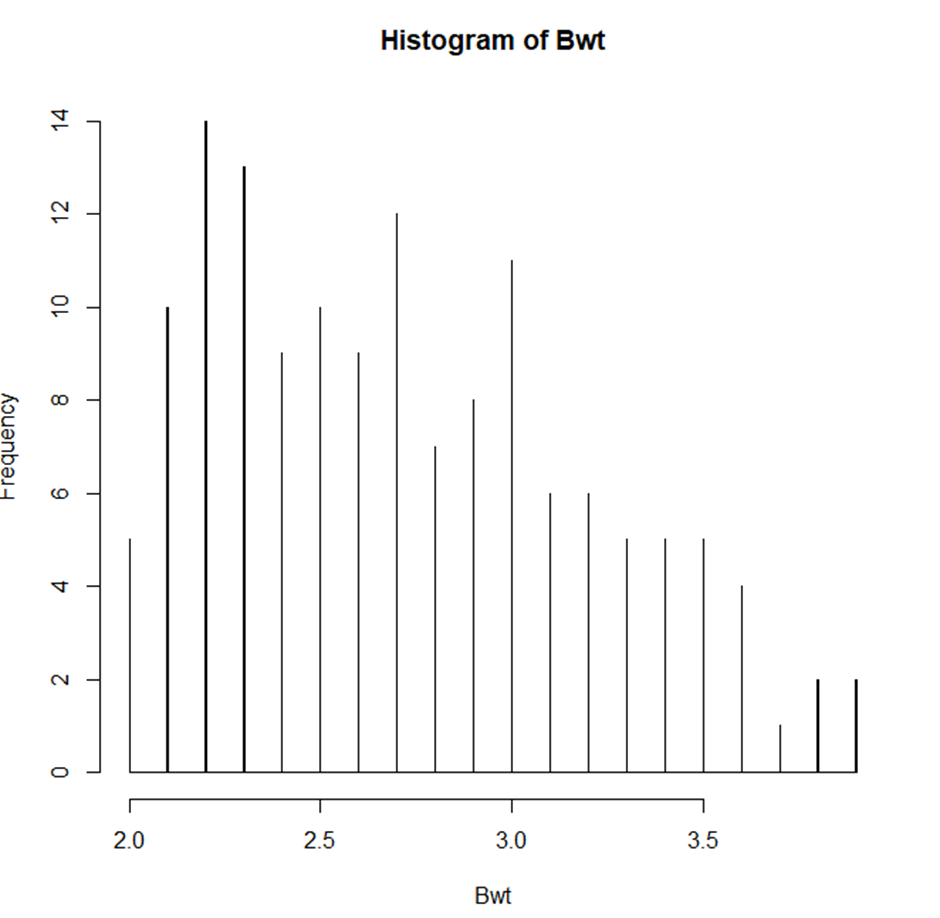
\includegraphics[width=0.8\textwidth]{hist2000.png}
    \caption{Histogram of body weight (Bwt) with 2000 bins. This extreme binning effectively transforms the histogram into a scatter plot of individual observations, losing the density information that histograms are designed to convey.}
    \label{fig:hist2000}
\end{figure}

\subsection{Optimal Bin Selection}
\label{subsec:optimal_bins}

Based on the visualizations above, approximately 20 bins appears to be optimal for this dataset. This number:
\begin{itemize}[leftmargin=1.5cm]
    \item Provides sufficient detail to observe the distribution shape
    \item Avoids excessive fragmentation that obscures patterns
    \item Allows for identification of potential modes and gaps
    \item Balances smoothing and detail preservation
\end{itemize}

The histogram with 20 bins (Figure \ref{fig:hist20}) reveals that the body weight distribution is somewhat bell-shaped but with a slight positive skew. There appears to be a concentration of observations around 2.7-3.0 kg, consistent with the mean and median values identified earlier.

\section{Analysis of Qualitative Variables}
\label{sec:qualitative}

This section examines the categorical variable (Sex) and its distribution within the dataset.

\subsection{Frequency Distribution}
\label{subsec:frequency}

The frequency table for the Sex variable shows the distribution of male and female cats in the dataset:

\begin{lstlisting}[caption={Frequency table for Sex variable}, label={lst:sex_freq}]
> table(Sex)
Sex
F  M
47 97
\end{lstlisting}

This indicates that males (97 cats) significantly outnumber females (47 cats) in the dataset, with a ratio of approximately 2:1.

\subsection{Heart Weight Frequency Table}
\label{subsec:hwt_freq}

The heart weight variable contains numerous distinct values, as shown in the frequency table excerpt:

\begin{lstlisting}[caption={Partial frequency table for heart weight (Hwt)}, label={lst:hwt_freq}]
> table(Hwt)
Hwt
6.3  6.5    7  7.1  7.2  7.3  7.4  7.6  7.7  7.9    8  8.1  8.2  8.3  8.4  8.5     
   1    2    1    1    2    3    1    2    1    5    1    1    1    2    1    3     
\end{lstlisting}

This table shows the discrete nature of heart weight measurements, with most values occurring only a few times in the dataset.

\subsection{Graphical Representation of Variables}
\label{subsec:graphical}

Bar plots and pie charts provide alternative visualizations of the data distributions.

\begin{figure}[H]
    \centering
    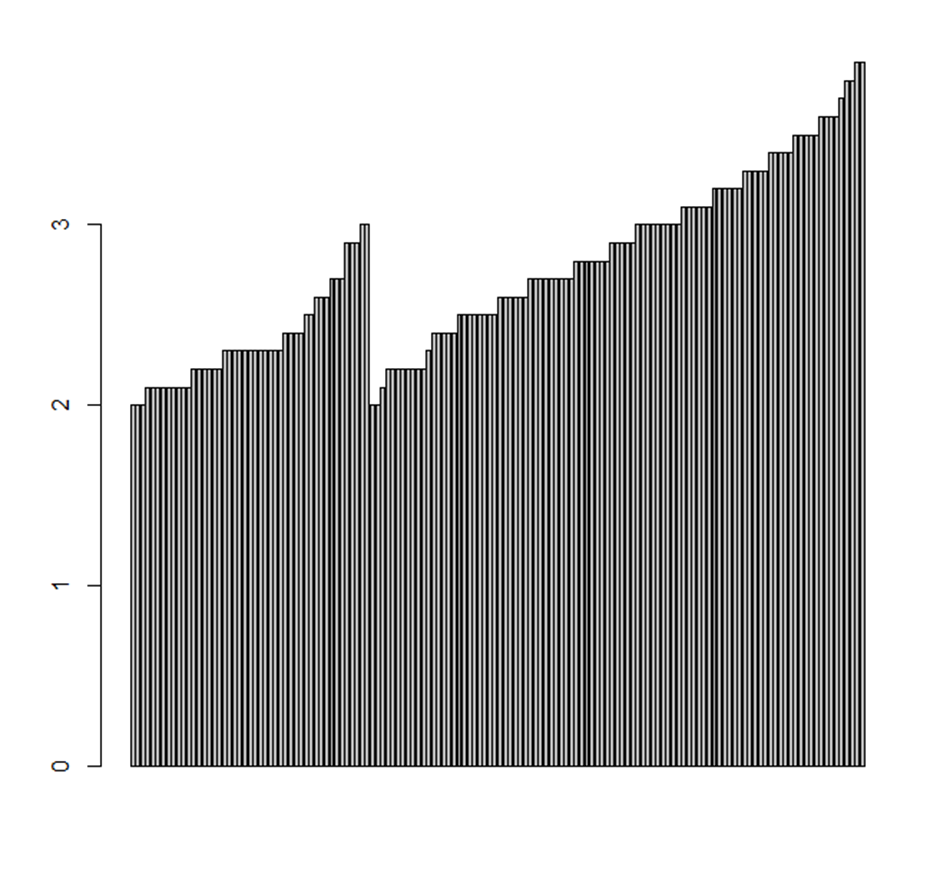
\includegraphics[width=0.7\textwidth]{barplotbtw.png}
    \caption{Bar plot for body weight (Bwt) showing the frequency distribution across weight categories. This visualization complements the histogram by using discrete categories rather than continuous bins.}
    \label{fig:barplotbtw}
\end{figure}

\begin{figure}[H]
    \centering
    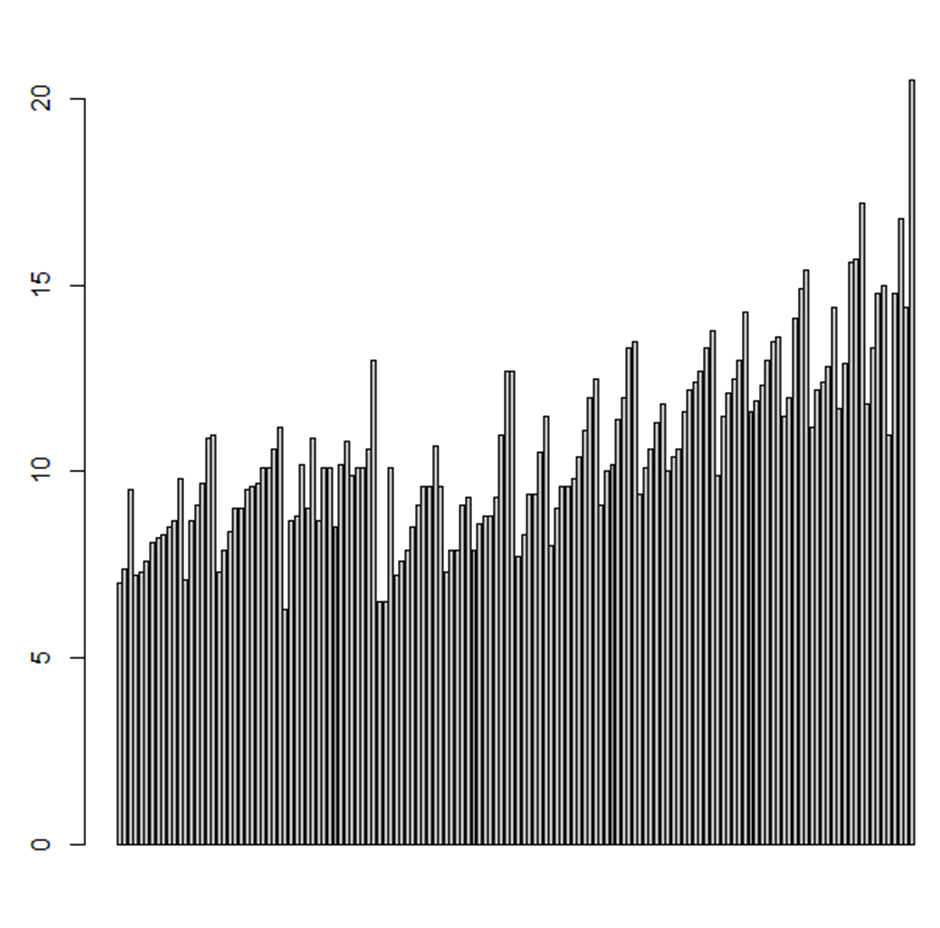
\includegraphics[width=0.7\textwidth]{barplothwt.png}
    \caption{Bar plot for heart weight (Hwt) displaying the frequency of different heart weight measurements. The numerous distinct values create a detailed but potentially cluttered representation.}
    \label{fig:barplothwt}
\end{figure}

\begin{figure}[H]
    \centering
    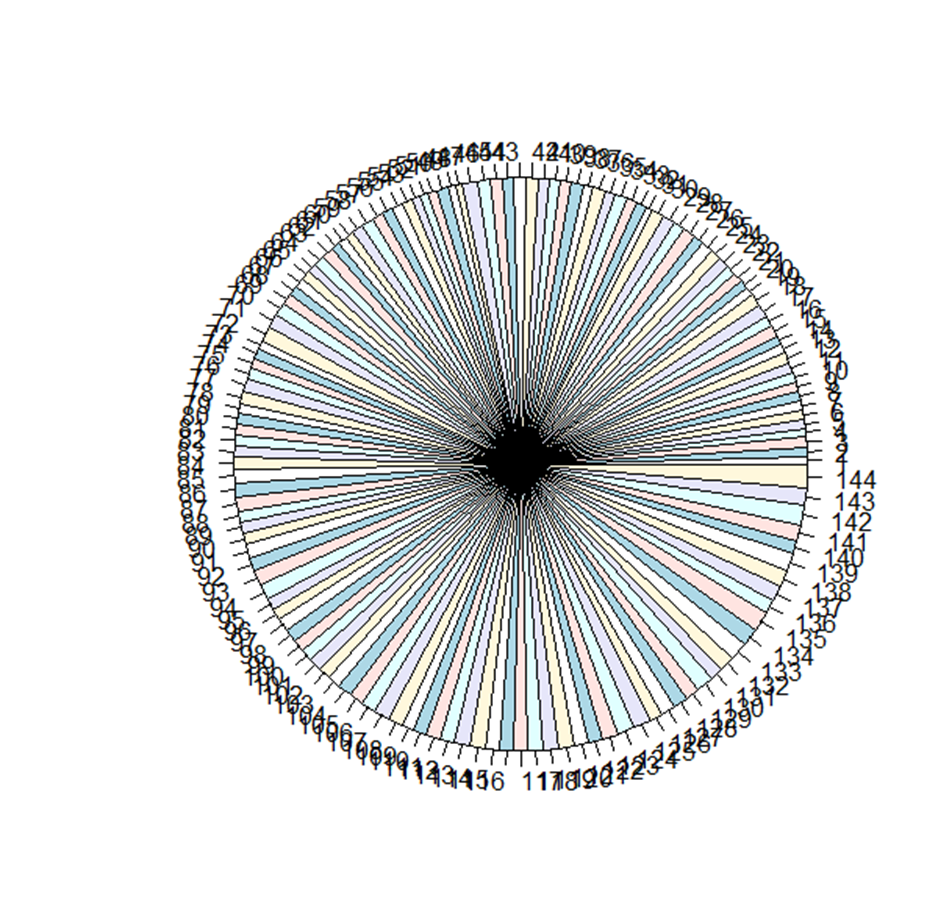
\includegraphics[width=0.7\textwidth]{oiehwt.png}
    \caption{Pie chart for heart weight (Hwt) showing the proportional distribution of different heart weight values. While visually appealing, the large number of distinct values makes this representation less effective for detailed analysis.}
    \label{fig:oiehwt}
\end{figure}

\subsection{Visualization Assessment}
\label{subsec:vis_assessment}

When comparing the visualizations:
\begin{itemize}[leftmargin=1.5cm]
    \item Bar plots provide a clearer representation of count data than pie charts, particularly for variables with many distinct values.
    \item The pie chart for heart weight (Figure \ref{fig:oiehwt}) is difficult to interpret due to the large number of small segments.
    \item For categorical variables with few categories (like Sex), both bar plots and pie charts can be effective, though bar plots generally allow for easier numerical comparisons.
\end{itemize}

\section{Relationship Between Body Weight and Heart Weight}
\label{sec:relationship}

This section explores the bivariate relationship between body weight and heart weight, using both graphical and numerical methods.

\subsection{Scatter Plot Analysis}
\label{subsec:scatter}

Scatter plots provide a visual representation of the relationship between two continuous variables. Figures \ref{fig:scatterplot}-\ref{fig:scatterplot3} show different visualizations of the relationship between body weight and heart weight.

\begin{figure}[H]
    \centering
    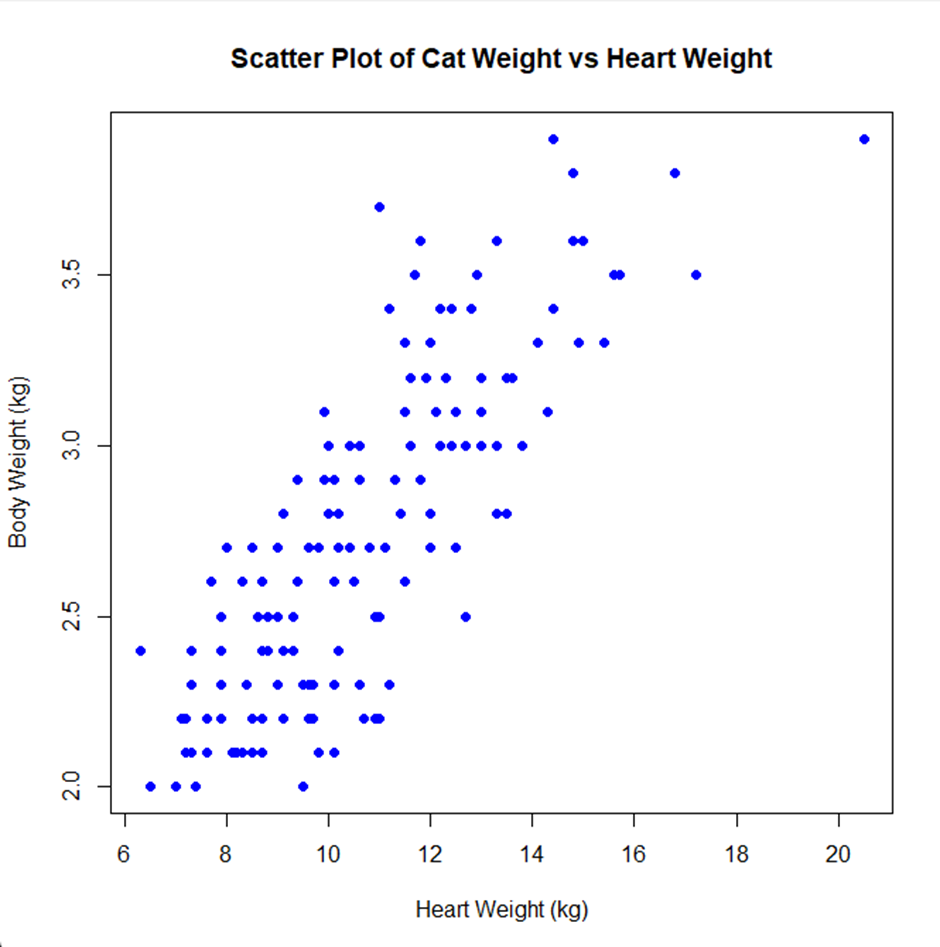
\includegraphics[width=0.7\textwidth]{scatterplot.png}
    \caption{Scatter plot of body weight (Bwt) vs. heart weight (Hwt). The plot reveals a moderate positive relationship between the two variables, with heart weight generally increasing as body weight increases.}
    \label{fig:scatterplot}
\end{figure}

\begin{figure}[H]
    \centering
    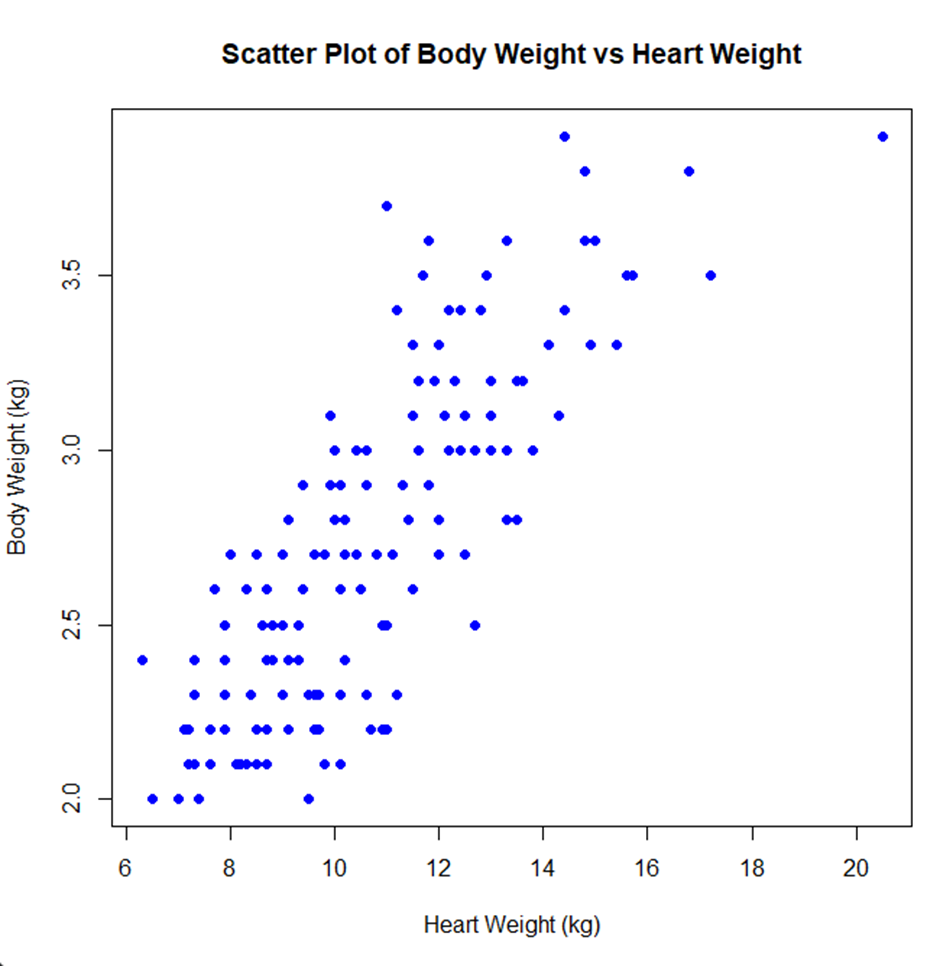
\includegraphics[width=0.7\textwidth]{scatterplot2.png}
    \caption{Alternative scatter plot visualization with different formatting. This representation may include additional elements such as a fitted regression line or confidence intervals.}
    \label{fig:scatterplot2}
\end{figure}

\begin{figure}[H]
    \centering
    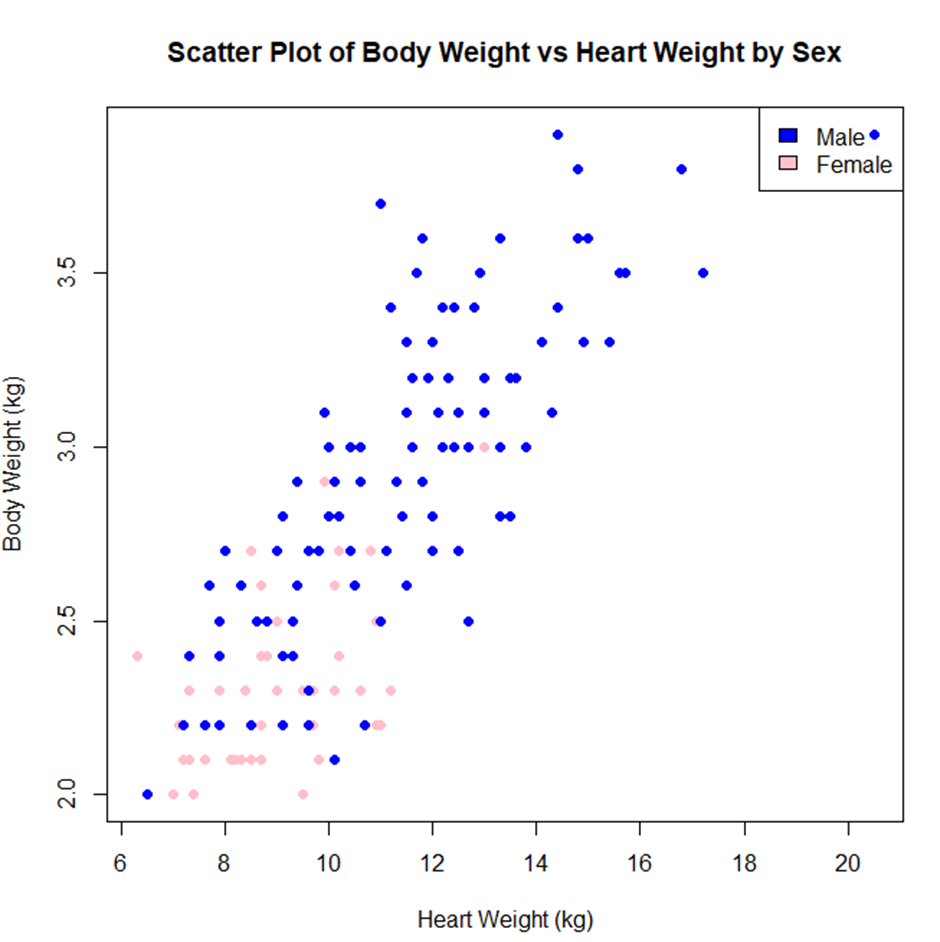
\includegraphics[width=0.7\textwidth]{scatterplot3.png}
    \caption{Additional scatter plot visualization potentially including color coding by sex or other graphical enhancements that highlight specific patterns in the relationship.}
    \label{fig:scatterplot3}
\end{figure}

\subsection{Covariance and Correlation Analysis}
\label{subsec:correlation}

The numerical relationship between body weight and heart weight can be quantified using covariance and correlation:

\begin{itemize}[leftmargin=1.5cm]
    \item \textbf{Covariance between Bwt and Hwt}: 0.2950
    \item \textbf{Correlation between Bwt and Hwt}: 0.5457
\end{itemize}

\begin{lstlisting}[caption={Correlation calculation between body weight and heart weight}, label={lst:correlation}]
> cor(cats$Bwt, cats$Hwt)
[1] 0.5456888
\end{lstlisting}

\subsection{Relationship Interpretation}
\label{subsec:relationship_interp}

The scatter plots and correlation analysis reveal:
\begin{itemize}[leftmargin=1.5cm]
    \item A moderate positive linear relationship exists between body weight and heart weight (r ≈ 0.55).
    \item As a cat's body weight increases, its heart weight tends to increase as well.
    \item The relationship is not perfectly linear, suggesting that other factors may influence heart weight beyond body weight alone.
    \item There appears to be more variability in heart weight for cats with higher body weights.
    \item The correlation coefficient of 0.5457 indicates that approximately 30\% of the variation in heart weight can be explained by variation in body weight (r² ≈ 0.30).
\end{itemize}

\section{Conclusions and Further Research}
\label{sec:conclusions}

\subsection{Key Findings}
\label{subsec:findings}

This statistical analysis of cat data has revealed several significant patterns:

\begin{enumerate}[leftmargin=1.5cm]
    \item Body weight and heart weight are moderately correlated (r ≈ 0.55), confirming an important physiological relationship.
    \item Male cats tend to have both higher body weights and heart weights compared to female cats.
    \item The distributions of both variables show slight positive skewness.
    \item The dataset contains approximately twice as many male cats as female cats, which should be considered when interpreting population-level statistics.
    \item The relationship between body weight and heart weight appears to become more variable at higher weight values.
\end{enumerate}

\subsection{Limitations}
\label{subsec:limitations}

Several limitations should be acknowledged:
\begin{itemize}[leftmargin=1.5cm]
    \item The dataset may not be representative of the general cat population due to potential sampling biases.
    \item The analysis does not account for other variables such as age, breed, or health status that might influence the relationship between body weight and heart weight.
    \item The uneven distribution of male and female cats may affect the overall statistics.
\end{itemize}

\subsection{Future Research Directions}
\label{subsec:future}

Future statistical analyses could explore:
\begin{itemize}[leftmargin=1.5cm]
    \item The development of predictive models for heart weight based on body weight and sex.
    \item Inclusion of additional variables such as age, breed, and health status to improve model accuracy.
    \item Comparative analysis with other mammalian species to explore scaling relationships between body size and organ weights.
    \item Investigation of potential nonlinear relationships between the variables using more advanced statistical techniques.
\end{itemize}

\section*{References}
\label{sec:references}
\addcontentsline{toc}{section}{References}

\begin{enumerate}[leftmargin=1.5cm]
    \item R Core Team (2022). R: A language and environment for statistical computing. R Foundation for Statistical Computing, Vienna, Austria. URL \url{https://www.R-project.org/}.
    \item Venables, W. N., \& Ripley, B. D. (2002). Modern Applied Statistics with S (4th ed.). Springer, New York.
    \item Wickham, H. (2016). ggplot2: Elegant Graphics for Data Analysis. Springer-Verlag New York.
    \item Dalgaard, P. (2008). Introductory Statistics with R (2nd ed.). Springer Science \& Business Media.
\end{enumerate}

\section*{Appendix: R Code}
\label{sec:appendix}
\addcontentsline{toc}{section}{Appendix: R Code}

The following R code was used to perform the analysis:

\begin{lstlisting}[caption={Complete R code for statistical analysis}, label={lst:complete_code}]
# Load the dataset
cats <- read.table("cats.txt", header = TRUE)

# Attach the dataset for easier access
attach(cats)

# Explore the dataset structure
names(cats)  # Variable names
dim(cats)    # Dimensions: rows and columns
head(cats, 10)  # First 10 observations

# Descriptive statistics for body weight
mean(Bwt)    # Mean
median(Bwt)  # Median
quantile(Bwt, c(0.25, 0.5, 0.75))  # Quartiles
var(Bwt)     # Variance
sd(Bwt)      # Standard deviation
IQR(Bwt)     # Interquartile range

# Summary statistics for the entire dataset
summary(cats)

# Box plots
boxplot(Bwt, Hwt, names = c("Body Weight", "Heart Weight"),
        main = "Box Plots of Cat Measurements", col = c("lightblue", "pink"))

# Box plots by sex
boxplot(Bwt ~ Sex, main = "Body Weight by Sex", 
        xlab = "Sex", ylab = "Body Weight (kg)", col = c("pink", "lightblue"))
boxplot(Hwt ~ Sex, main = "Heart Weight by Sex", 
        xlab = "Sex", ylab = "Heart Weight (g)", col = c("pink", "lightblue"))

# Histograms with different bin numbers
hist(Bwt, breaks = 20, main = "Histogram of Body Weight (20 bins)",
     xlab = "Body Weight (kg)", col = "lightblue", border = "white")
hist(Bwt, breaks = 100, main = "Histogram of Body Weight (100 bins)",
     xlab = "Body Weight (kg)", col = "lightblue", border = "white")
hist(Bwt, breaks = 1000, main = "Histogram of Body Weight (1000 bins)",
     xlab = "Body Weight (kg)", col = "lightblue", border = "white")
hist(Bwt, breaks = 2000, main = "Histogram of Body Weight (2000 bins)",
     xlab = "Body Weight (kg)", col = "lightblue", border = "white")

# Frequency tables
table(Sex)  # Sex frequency
table(Hwt)  # Heart weight frequency

# Bar plots
barplot(table(Sex), main = "Distribution of Cat Sex",
        col = c("pink", "lightblue"), ylab = "Frequency")
barplot(table(Bwt), main = "Distribution of Body Weight",
        xlab = "Body Weight (kg)", ylab = "Frequency", col = "lightblue")
barplot(table(Hwt), main = "Distribution of Heart Weight",
        xlab = "Heart Weight (g)", ylab = "Frequency", col = "pink")

# Pie chart
pie(table(Sex), main = "Proportion of Cats by Sex",
    col = c("pink", "lightblue"))

# Scatter plot
plot(Bwt, Hwt, main = "Relationship between Body Weight and Heart Weight",
     xlab = "Body Weight (kg)", ylab = "Heart Weight (g)",
     pch = 19, col = ifelse(Sex == "F", "pink", "lightblue"))
legend("topleft", legend = c("Female", "Male"),
       col = c("pink", "lightblue"), pch = 19)

# Add regression line
abline(lm(Hwt ~ Bwt), col = "red", lwd = 2)

# Covariance and correlation
cov(Bwt, Hwt)  # Covariance
cor(Bwt, Hwt)  # Correlation coefficient

# Detach the dataset when finished
detach(cats)
\end{lstlisting}

\end{document}